\subsection{TCP connecties beveiligen: SSL en TLS}

\subsubsection{SSL = Secure Sockets Layer}

\textcolor{red}{\textbf{Secure Sockets Layer (SSL)}}=  Uitgebreide TCP die gebruik maakt van cryptografie

\begin{multicols}{2}
\bi
\itf widely deployed security protocol

\bi
\itf supported by almost all browsers, web servers
\itf https
\itf billions \$/year over SSL
    \ei

    \itf implementation: Netscape
    \itf variation -TLS: transport layer security, RFC 2246
    \itf provides

    \bi
    \itf confidentiality
    \itf integrity
    \itf authentication
    \ei
\ei
\end{multicols}


\begin{itemize}
\item \textbf{original goals}:
    \begin{itemize}
    \item Web e-commerce transactions 
    \item encryption (especially credit-card numbers)
    \item Web-server authentication
    \item optional client authentication
    \item minimum hassle in doing business with new merchant
    \end{itemize}
\item available to all TCP applications
    \begin{itemize}
    \item secure socket interface
    \end{itemize}
\end{itemize}


\noindent Op de transport laag kijken hoe cryptografie TCP kan versterken met beveiligingsdiensten. Deze verbeterde versie van TCP is beter bekend als \textbf{Secure Socket Layer (SSL)}. Een enigszins gewijzigde versie van SSL versie 3, wordt de \textbf{Transport Layer Security (TLS}) genoemd.

\noindent Het SSL protocol is ontworpen door Netscape. SSL wordt veel geïmplementeerd en wordt door alle populaire web browsers en servers ondersteund. Elk jaar worden er biljoenen uitgegeven aan SSL.

\begin{figure}[h]
    \centering
    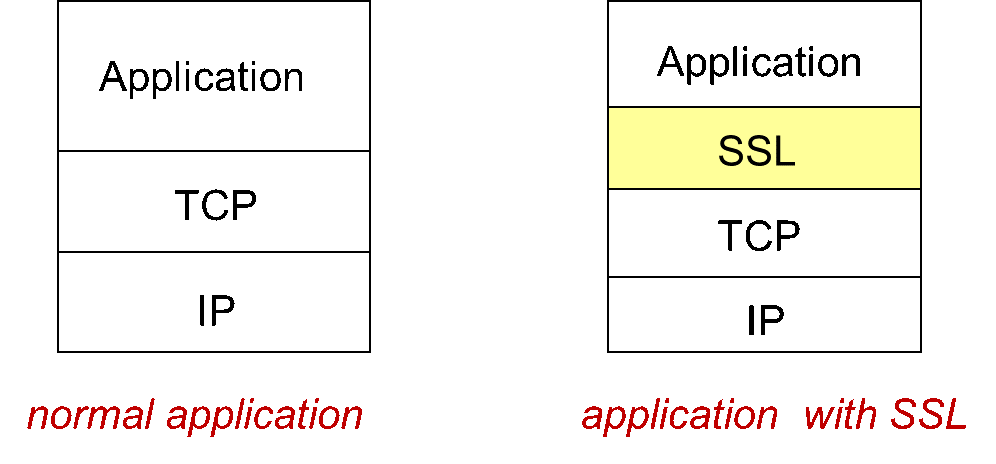
\includegraphics[width=2in]{./img/imghfdst8/hfdst8puntje27.png}
    \caption{ }      
    \label{fig: }
\end{figure}

\noindent SSL verbetert TCP door te zorgen dat er confidentialiteit, data integriteit, server en client authenticatie is. Omdat SSL TCP beveiligd, kan het worden gebruikt door eender welke applicatie die TCP gebruikt.

\subsubsection{TLS = Transport Layer Security}

\textcolor{red}{\textbf{Transport Layer Security (TLS):}} Een iets gewijzigde versie van SSL

\clearpage

\subsubsection{Het grote plaatje}

\noindent Eerst een eenvoudige versie van SSL beschrijven. Dit gaan we de Almost-SSL noemen. Almost-SSL en SSL hebben vier fasen: de handshake, key derivation, data transfer en connectie sluiten.

\subsubsubsection{Handshake}

\be
\itf P1: SYN, P2: SYNACK, P1: ACK
\itf P1 stuurt een SSL-hello-bericht waarop hij het certificaat van P2 krijgt.
\itf P1 genereert een mastersleutel en versleutelt deze sleutel met de publieke sleutel van P2
\ee

\begin{figure}[h]
    \centering
    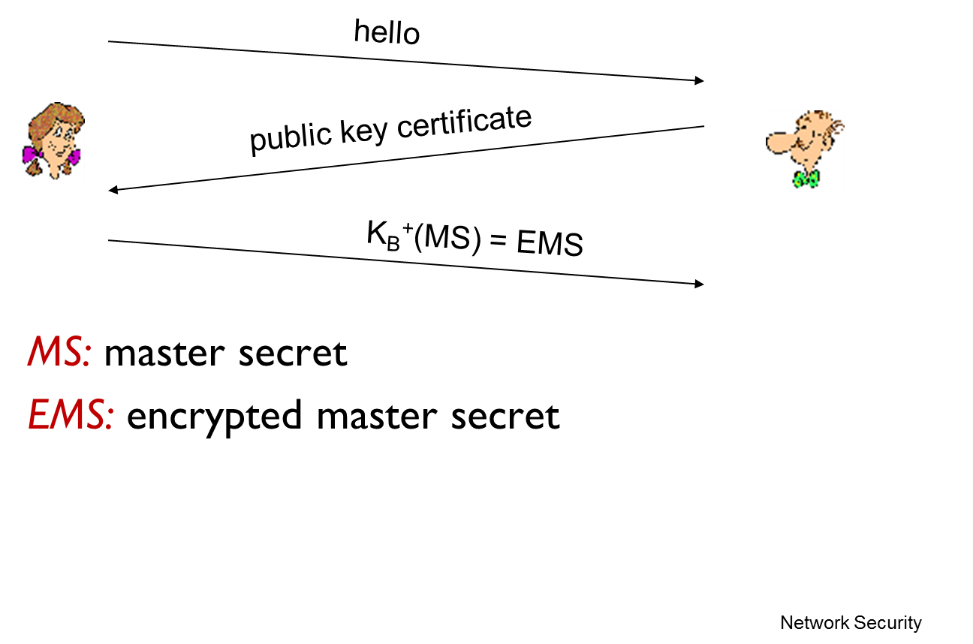
\includegraphics[width=4in]{./img/imghfdst8/hfdst8puntje28.png}
    \caption{ }      
    \label{fig: }
\end{figure}

\noindent Gedurende de handshake fase, heeft Bob behoefte aan een TCP connectie op te zetten met Alice, bevestigen dat Alice echt Alice is, en vervolgens Alice de master secret key te sturen die gebruikt zal worden om bij Alice en Bob de symmetrische sleutels te genereren die ze nodig hebben voor de SSL sessie.

\noindent Wanneer de TCP connectie opgezet is, zend Bob naar Alice een hallo bericht. Alice reageert met haar certificaat, die haar publieke sleutel bevat. Bob genereert vervolgens een Master Secret (MS) die enkel gebruikt gaat worden voor deze SSL sessie, ecrypteerd de MS met de publieke sleutel van Alice om zo de \textbf{Encrypted Master Secret (EMS)} te maken, en zendt deze dan door naar Alice. Alice decrypteerd het EMS met haar prive sleutel. Na deze fase kennen enkel Bob en Alice de MS voor deze SSL sessie.

\clearpage

\subsubsubsection{Key derivation = het verkrijgen van een sleutel}

\noindent Gebruik verschillende sleutels voor de Message Authentication Code (=\textbf{HMAC}) en encryptie

\noindent Message authenticaton code: HMAC with shared key H(m+s)

\noindent Er worden 4 verschillende sleutels gegenereerd uit de mastersleutel (=\textbf{MS}), namelijk:
\begin{itemize}
\item $E_B$ = sessie encryptie sleutel voor data die verzonden wordt van Bob naar Alice
\item $M_B$ = sessie MAC sleutel voor data die verzonden wordt van Bob naar Alice
\item $E_A$ = sessie encryptie sleutel voor data die verzonden wordt van Alice naar Bob
\item $M_A$ = sessie MAC sleutel voor data die verzonden wordt van Alice naar Bob
\end{itemize}

\noindent Dit kan gedaan worden door gewoon de MS te splitsen in \textbf{vier} sleutels. Op het einde van deze fase hebben Alice en Bob elk alle vier sleutels. De twee encryptie sleutels gaan gebruikt worden om de data te encrypteren. De twee MAC sleutels worden gebruikt om de integriteit van de data te controleren.

\subsubsubsection{Data transfer}


De gegevensstream wordt opgesplitst in \textbf{records}. SSL voegt een \textbf{berichtauthenticatiecode} (\textbf{MAC}) toe aan elke record.

\fra  Connection closure:Speciale berichten om de connectie veilig te sluiten.

\noindent Sinds TCP een byte stream protocol is, zou een natuurlijke benadering voor SSL zijn om de applicatie data on the fly te encrypteren en vervolgens de geëncrypteerde data on the fly door te geven aan TCP. Maar als we dit doen, waar zouden we MAC zetten voor de integriteit check?
SSL breekt de data stroom in verschillende records, voegt een MAC toe aan elk record voor integriteit controle en encrypteerd vervolgens de record+MAC. Om de MAC te maken voegt Bob de record data met de sleutel MB toe in een hash functie. Om het pakket te encrypteren gebruikt Bob zijn sessie sleutel $E_B$. Dit geëncrypteerde pakket wordt dan doorgestuurd naar TCP voor transport over het internet.
Maar er is nog een probleem. Een indringer heeft de mogelijkheid om segmentent toe te voegen, vervangen en te verwijderen. Bijvoorbeeld, een indringer vangt twee pakketten die verzonden zijn door Bob, en vervangt de TCP sequentie nummers (die niet geëncrypteerd zijn), en verzend deze omgewisselde segmenten door naar Alice.
De gedecrypteerde byte stream gaat niet in de juiste volgerde staan, en zal dus niet de juiste informatie weergeven.

\noindent De oplossing voor dit probleem is om \textbf{sequentie nummers} te gebruiken. SSL doet dit als volgt. Bob onderhoud een sequentie nummer teller, die bij nul begint en wordt verhoogt bij elke SSL record dat hij stuurt. Bob voegt niet echt een sequentie nummer toe aan de record zelf, maar wanneer hij de MAC berekent, voegt hij het sequentie nummer toe bij MAC berekening. Dus \textcolor{red}{MAC is nu een hash van data + de MAC sleutel $M_B$ + de huidige sequentie nummer.}
Alice volgt Bob zijn sequentie nummers, wat haar toe laat om de data integriteit met de passende sequentie nummer van een record te controleren.
Een indringer kan nog altijd heel de communicatie opnieuw afspelen. Oplossing hiervoor is om een \textbf{nonce} te gebruiken.

\clearpage

\subsubsubsection{SSL record}

De SSL record bestaat uit de volgende velden:
\begin{itemize}

\item Type
\item Versie
\item Lengte
\item Data
\item MAC
\end{itemize}

\noindent De eerste 3 velden zijn niet geëncrypteerd. Deze velden tonen aan of de record een handshshake bericht is of een bericht dat applicatie data bevat. Het wordt ook gebruikt om de SSL connectie te sluiten. De lengte is om de SSL records uit de TCP byte stream te krijgen.

\clearpage

\subsubsection{Een iets completer beeld}

\subsubsubsection{SSL Handshake}

\noindent Alice en Bob mogen aan het begin van een SSL-sessie zelf afspreken welke versleutelingsalgoritmen ze willen gebruiken. \fra deze fase heet de \textbf{handshake} fase. 

\noindent Hiernaast zenden Alice en Bob nonces naar elkaar toe, die gebruikt zullen worden voor het aanmaken van de sessiesleutels ($E_B$ , $M_B$ , $E_A$ en $M_A$ ).

Dan de stappen van de echte SSL handshakeprocedure zijn:

\begin{enumerate}

\item De client verzendt een lijst met versleutelingsalgoritmen die hij ondersteunt en een zelfgekozen nonce.
\item Uit deze ontvangen lijst gaat de server algoritmes kiezen meer specifiek:

\be
\itf Een algoritme voor de symmetrische sleutel vb. AES
\itf Een algoritme voor de publieke sleutel vb. RSA
\itf Een algoritme voor de berichtauthenticatiecode (MAC = Message Authentication Code).

\ee
Vervolgens stuurt de server een bericht terug naar de client, samen met zijn voorkeuren, een certificaat en een zelfgekozen nonce.

\item De client:

\be
\itf Authenticeert het certificaat
\itf Berekent de publieke sleutel van de server
\itf Genereert een geheime pre-mastersleutel (PMS)
\itf Versleutelt de PMS met de publieke sleutel van de server
\itf Verzendt de versleutelde PMS naar de server.
\ee

\item Gebruik makend van dezelfde key derivation functie, gaan de client en server onafhankelijk van elkaar de Master Secret berekenen van de PMS en nonces. De MS is vervolgens opgedeeld om twee encryptie en twee MAC sleutels te genereren. Bovendien wanneer de symmetrische cipher CBC gebruikt, worden er twee Initialisatie Vectors (VI) verkregen uit de MS. Voortaan zijn alle berichten verzonden tussen de client en server geëncrypteerd en geauthentificeerd (met de MAC).
\item De client verzend een MAC van alle handshake berichten.
\item De server verzend een MAC van alle handshake berichten.
\end{enumerate}

\noindent De laatste twee stappen beschermen de handshake van geknoei.

\noindent Bij stap 1 wordt een lijst van algoritmes doorgestuurd in cleartext. Een indringer kan de sterkere algoritmes uit de lijst halen zodat de server een zwakker algoritme gaat kiezen. 

Om zo’n geknoei te voorkomen, wordt in stap 5 voor de client een MAC met een aaneenschakeling van alle handshake berichten gemaakt die verzonden en ontvangen zijn. De server kan deze MAC controleren door op dezelfde manier te werk te gaan. Als er een tegenstrijdig signaal is, gaat de server de connectie onmiddellijk beëindigen. De server stuurt zijn berekende MAC terug naar de client zodat deze ook kan controleren op tegenstrijdigheden.

\noindent In SSL worden nonces gebruikt om zich te verdedigen tegen de connection replay attack en sequentie nummers worden gebruikt om zich te verdedigen tegen het hersturen van pakketten tijdens een open sessie.

\subsubsubsection{Connection closure}

Op een moment gaat Bob of Alice de SSL sessie afsluiten. Een benadering zou kunnen zijn dat Bob de SSL sessie beëindigd door de onderliggende TCP connectie af te sluiten, dat is als Bob een TCP FIN segment stuurt naar Alice. Maar zo’n ontwerp kan leiden naar een truncation attack waar een indringer een SSL sessie vroeger kan afsluiten.
De oplossing tot dit probleem is om aan te duiden in het type veld als de record dient om de SSL sessie af te sluiten. Het type veld word on-geëncrypteerd gestuurd en kan zo gelezen worden, maar wordt geauthenticeerd bij de ontvanger door gebruik te maken van de Record’s MAC. Dus als er eerst een TCP FIN gestuurd wordt voor een closure SSL record, kan men er van uitgaan dat er iets niet juist is.
